% ****** Start of file apssamp.tex ******
%
%   This file is part of the APS files in the REVTeX 4.2 distribution.
%   Version 4.2a of REVTeX, December 2014
%
%   Copyright (c) 2014 The American Physical Society.
%
%   See the REVTeX 4 README file for restrictions and more information.
%
% TeX'ing this file requires that you have AMS-LaTeX 2.0 installed
% as well as the rest of the prerequisites for REVTeX 4.2
%
% See the REVTeX 4 README file
% It also requires running BibTeX. The commands are as follows:
%
%  1)  latex apssamp.tex
%  2)  bibtex apssamp
%  3)  latex apssamp.tex
%  4)  latex apssamp.tex
%
\documentclass[%
 reprint,
 superscriptaddress,
%groupedaddress,
%unsortedaddress,
%runinaddress,
%frontmatterverbose, 
%preprint,
%preprintnumbers,
%nofootinbib,
%nobibnotes,
%bibnotes,
 amsmath,amssymb,
 aps, prl, twocolumn, showpacs,
%pra,
%prb,
%rmp,
%prstab,
%prstper,
%floatfix,
]{revtex4-2}

\usepackage{graphicx}% Include figure files
\usepackage{subcaption}
\usepackage{dcolumn}% Align table columns on decimal point
\usepackage{bm}% bold math
%\usepackage{hyperref}% add hypertext capabilities
%\usepackage[mathlines]{lineno}% Enable numbering of text and display math
%\linenumbers\relax % Commence numbering lines

%\usepackage[showframe,%Uncomment any one of the following lines to test 
%%scale=0.7, marginratio={1:1, 2:3}, ignoreall,% default settings
%%text={7in,10in},centering,
%%margin=1.5in,
%%total={6.5in,8.75in}, top=1.2in, left=0.9in, includefoot,
%%height=10in,a5paper,hmargin={3cm,0.8in},
%]{geometry}
\usepackage[justification=raggedright,singlelinecheck=false]{caption}
\usepackage{amsthm}
\usepackage{multirow}
\usepackage{array}
\usepackage{booktabs}
\usepackage{svg}
\newtheorem{theorem}{Theorem}
\newtheorem{corollary}{Corollary}[theorem]
\newtheorem{lemma}{Lemma}
\newtheorem{definition}{Definition}
\newtheorem{example}{Example}
\newtheorem{fact}{Fact}
\newtheorem{proposition}{Proposition}
\newtheorem{conjecture}{Conjecture}
\newcommand{\RomanNumeralCaps}[1]
    {\MakeUppercase{\romannumeral #1}}
\newcommand*{\dif}{\mathop{}\!\mathrm{d}}
\DeclareMathOperator*{\argmax}{argmax}

\begin{document}

\preprint{APS/123-QED}

% \title{A Universal Characterization of Trainability in Variational Quantum Algorithms}% Force line breaks with \\
\title{Beyond Unitary Designs: Quantifying Trainability in Parameterized Quantum Circuits}
% \thanks{A footnote to the article title}%

\author{Jinhong Zeng, Zhenyue Du, Zhaokai Li}
% \altaffiliation[Also at ]{Physics Department, University of Science and Technology of China.}
% Lines break automatically or can be forced with \\
% \author{Second Author}%
% \email{Second.Author@institution.edu}
%\affiliation{%
% Authors' institution and/or address\\
% This line break forced with \textbackslash\textbackslash
% }%

% \collaboration{MUSO Collaboration}%\noaffiliation

% \author{Charlie Author}
% \homepage{http://www.Second.institution.edu/~Charlie.Author}
% \affiliation{
% Second institution and/or address\\
% This line break forced% with \\
% }%
% \affiliation{
% Third institution, the second for Charlie Author
% }%
% \author{Delta Author}
% \affiliation{%
% Authors' institution and/or address\\
% This line break forced with \textbackslash\textbackslash
% }%%

%\collaboration{CLEO Collaboration}%\noaffiliation

\date{\today}% It is always \today, today,
             %  but any date may be explicitly specified

\begin{abstract}
% Variational quantum algorithms are promising for noisy intermediate-scale quantum devices; yet, their performance is often limited by exponentially vanishing gradients. 
% While much research has examined the trainability of specific circuit structures, a systematic framework has been lacking. 

Parameterized quantum circuits (PQCs) represent a central class of controllable quantum evolutions, yet their trainability can be severely limited by exponentially vanishing gradients, known as the barren plateau phenomenon. Existing analyses typically rely on strong randomness assumptions, such as unitary designs and remain limited in addressing general structured circuits.
% , a systematic framework to characterize the trainability of arbitrary PQCs remains lacking.
In this Letter, we develop a measure-based framework to characterize the trainability of general PQCs and establish a level classification of gradient variance across orthogonal subspaces. Our results reveal a trainability advantage in previously unexplored unitary 1-designs compared to higher-order designs. We further introduce the improvement potential to quantify maximal variance enhancement under local disturbances. This framework provides unified analytical guidance for understanding and engineering trainable quantum circuits on near-term quantum hardware.

% In this Letter, we develop a measure-based framework to characterize the trainability of arbitrary PQCs by approximating circuit-induced measures with polynomial probability measures. This enables a level classification of trainability across orthogonal subspaces and uncovers a trainability advantage in previously overlooked unitary 1-designs. We further introduce the improvement potential to quantify maximal variance enhancement under local disturbances, providing guidance for designing more trainable PQCs. Our results establish a unified theoretical foundation for the optimization landscape of controllable quantum devices.
% to characterize trainability across different architectures. Any probability measure induced by a quantum circuit can be approximated to arbitrary precision within our measure class, with bounded deviation in gradient variance. This framework enables the classification of barren plateau phenomena across orthogonal subspaces, refines existing theoretical bounds, and yields an improved criterion for assessing trainability, illustrated through parameterized quantum circuit examples.


% \begin{description}
% \item[Usage]
% Secondary publications and information retrieval purposes.
% \item[Structure]
% You may use the \texttt{description} environment to structure your abstract;
% use the optional argument of the \verb+\item+ command to give the category of each item. 
% \end{description}
\end{abstract}

%\keywords{Suggested keywords}%Use show-keys class option if keyword
                              %display desired
\maketitle

%\tableofcontents

% Quantum computation has made remarkable advancements due to significant theoretical and experimental research over the past decades. Many researchers have demonstrated quantum speed-up advantages across various applications~\cite{daley2022practical, huang2022quantum, bravyi2018quantum, lee2023evaluating, arvidsson2020quantum}. Yet, current devices remain in the noisy intermediate-scale quantum (NISQ) regime, constrained by limited qubit counts and imperfect gate fidelities~\cite{preskill2018quantum, lau2022nisq}. Variational quantum algorithms (VQAs) have become a promising method due to their low requirements for qubit counts and gate fidelities. A VQA combines a parameterized quantum circuit (PQC), defining the ansatz and cost function, with a classical optimizer that updates the circuit parameters. However, many PQCs exhibit vanishing gradients exponentially during training~\cite{mcclean2018barren,wang2021noise}, which severely affects the convergence of cost functions. Characterizing the trainability in VQAs, therefore, becomes a central issue.
After decades of development, quantum technology has demonstrated explicit advantages in areas such as accelerated computing and precision measurement~\cite{daley2022practical, huang2022quantum, bravyi2018quantum, lee2023evaluating, arvidsson2020quantum}. As a trainable framework for realizing such advantages, PQCs have become a widely used architecture for qubit computation and evolution, with notable applications in quantum metrology \cite{liu2024optimal,munoz2024photonic,de2025improving,yang2025programmable} and variational quantum algorithms (VQAs)~\cite{haug2022natural,miao2024neural,tilly2022variational,wu2023quantumdarts}. PQC's ability to solve given problems stems from its tunable internal parameters, which allow us to optimize them within a fixed ansatz to accomplish tasks. In practical applications, such optimization is typically achieved using gradient descent and its variants. However, it has been shown that for a broad class of parametrized quantum circuits, particularly those that are universal, the gradient of the cost function will vanish exponentially with the size of the system\cite{holmes2022connecting,gong2024enhancing}, resulting in severe trainability issues and degraded optimization performance, known as the barren plateau. Therefore, for a given PQC architecture, evaluating the probability of its gradients vanishing exponentially under the current parameter distribution is a crucial topic in the study of circuit trainability.
% The original progress of the research on the trainability of VQAs comes after the introduction of unitary designs~\cite{gross2007evenly,roy2009unitary}. A unitary $t$-design is a set of unitary matrices that statistically mimics the average ensemble over unitary groups up to the $t$-th moment, which is a suitable object to describe the expectation and variance of gradients of PQCs. The $\gamma$-approximate unitary 2-design exists widely in PQCs with sufficient randomness for $\gamma$ exponentially small~\cite{roy2009unitary}. It is known that a sufficiently random PQC can realize a $\gamma$-approximate unitary 2-design within $\mathcal{O}(n)$ circuit depth ($n$ is the number of qubits)~\cite{dankert2009exact}. Because unitary 2-designs accurately approximate the statistical behavior of large and well-randomized circuits, local structures based on unitary 2-designs~\cite{holmes2022connecting, pesah2021absence, park2024hamiltonian, cerezo2021cost} have become standard assumptions in recent research.

 Gradient variance is widely used as a standard indicator of gradient vanishing. By Chebyshev’s inequality, a small gradient variance implies a high probability of vanishing gradients\cite{mcclean2018barren}, which reduces the trainability problem to the evaluation of gradient variances under a specified parameter distribution. Most existing studies evaluate gradient variances under the unitary 2-design assumption\cite{cerezo2021cost,ortiz2021entanglement,fontana2024characterizing,cunningham2025investigating}, where a unitary $t$-design denotes an ensemble of unitary operators whose statistical moments up to order $t$ coincide with those of the Haar random measure. The Haar measure enables a precise evaluation of gradients for circuits that approximate a global unitary 2-design. However, this assumption is only satisfied by PQCs with strong randomness. Such circuits exhibit gradient variances scaling as $d^{-2}$(with Hilbert space dimension $d$), leading to exponentially flat optimization landscapes and poor convergence. For circuits that do not satisfy this assumption, a reliable analytical framework remains lacking.
 Recent research has extended this analytical framework to cover circuits composed of multiple local unitary 2-designs; nevertheless, each local 2-design remains constrained by the strong randomness assumption\cite{pesah2021absence, schumann2024emergence}.
 %Recent research has extended this analytical framework to circuits composed of multiple local unitary 2-designs, yet each local 2-design in this approach remains constrained by strong randomness assumptions.
 %PQCs with strong randomness typically approximate a unitary 2-design, where a unitary $t$-design denotes an ensemble of unitary operators whose statistical moments up to order $t$ coincide with those of complete randomness. Most existing studies evaluate gradient variances under the unitary 2-design assumption. However, such circuits exhibit gradient variances scaling as $d^{-2}$(with Hilbert space dimension $d$), leading to exponentially flat optimization landscapes and poor convergence. Recent work has extended this framework to local unitary 2-designs, enlarging the class of analyzable circuits, but the approach remains fundamentally constrained by strong randomness assumptions on PQCs.

%Although the local unitary 2-design assumption is reasonable for PQCs with sufficient randomness, it does not hold well in many cases within the NISQ era~\cite{holmes2022connecting}.  Additionally, for efficient PQCs tailored to specific problems, the local unitary 2-design assumption often fails to provide an accurate description of the system. As a result, it is hard to build a unified framework for all PQCs under this assumption. Even for unitary 1-designs, central to our zero-bias network study, a unified framework remains unattainable. Consequently, there is no clear level classification of trainability based on the structure of PQCs. A more general framework capable of adapting to all PQCs is necessary to overcome these limitations.

%In the NISQ era, most practical PQCs used in training lack sufficient strong randomness to approximate unitary designs effectively. Moreover, when partial structural information about the problem is available, it is commonly exploited to design tailored, problem-specific quantum circuits. 

In practice, quantum circuits are often designed with tailored structures for specific problems,  yet they typically lack sufficient randomness and thus fall outside the scope of existing analytical frameworks.
Since such non-random PQCs play a central role in practical quantum circuit design and applications, it is essential to develop a general, computable gradient variance framework that can adapt to all types of PQCs.

In this Letter, we develop a measure-based framework to characterize the trainability of PQCs beyond the standard unitary design paradigm. 
By introducing a class of polynomial probability measures, we prove that the distribution of any PQC can be approximated with arbitrary precision while preserving its gradient variance.
% (Propositions~\ref{prop: approx} and~\ref{prop: inv}). 
% that approximates any circuit-induced distribution to arbitrary precision, with bounded deviation in gradient variance (cf. Propositions~\ref{prop: approx} and~\ref{prop: inv}). 
Using zonal polynomials and Weingarten calculus~\cite{weingarten1978asymptotic, collins2003moments, collins2006integration}, we obtain explicit variance expressions and establish a level classification of trainability across orthogonal subspaces (Theorem~\ref{thm:1}).
% As an example, we investigate the previously overlooked unitary 1-designs by ?. 
% As an example, it gives the upper bound for previously overlooked unitary 1-designs (bypassing barren plateaus?)
% we obtain explicit variance expressions, thereby establishing a comprehensive theory on the trainability of arbitrary PQCs.
% Served as a bridge, it provides a level classification of trainability on PQCs from a measure perspective(cf. Theorem~\ref{thm:1}). 
% We construct a family of measures representing the unitary 1-design in Proposition~\ref{prop:1-design}. It provides a tight upper bound of the barren plateaus landscape of the unitary 1-design, which cannot be calculated under the previous unitary 2-design framework.
In particular, this framework identifies a significant trainability advantage in previously overlooked unitary 1-designs compared to higher-order designs. 
Furthermore, we define the concept of improvement potential to quantify the maximal variance enhancement achievable under local disturbance (Theorem~\ref{thm:potential}), thereby providing a criterion for designing more trainable PQCs. These results provide analytical guidance to identify and enhance the trainability of parameterized quantum circuits in the noisy intermediate-scale quantum(NISQ) era.
% Rich examples are provided to illustrate the potential of various circuits. 
% Finally, we employ numerical simulations to corroborate our analytical predictions.
% In this Letter, we have established a measure-theoretic framework based on balanced polynomial measures to characterize the trainability of PQCs. We proved that balanced polynomial measures with arbitrary precision can approximate any PQC via a global phase trick. Within this framework, we propose a variance contribution derived from zonal polynomial decomposition. In particular, we rigorously prove a tight upper bound on the gradient variance for unitary 1-designs. Numerical simulations for a two-qubit system corroborate our theoretical predictions. As an additional application, we introduce the concept of improvement potential and provide an explicit criterion for evaluation, with examples demonstrating both negligible and significant enhancements. Overall, our results reveal the measure-level factors that govern trainability and provide guiding principles for designing more trainable PQCs.
% Future research may benefit from integrating balanced polynomial measures with tools from dynamical Lie algebra theory~\cite{diaz2023showcasing, ragone2024lie}, potentially leading to a more practical and comprehensive analytical framework.

\emph{\label{sec:2} Preliminaries.}---
The performance of VQAs is related to the selected ansatz in the training. Generally, an ansatz consists of a PQC $U(\boldsymbol\theta)$, and a cost function $C(\boldsymbol\theta)$ with trainable parameters $\boldsymbol\theta$. Since trainability depends on the type of selected ansatz, we adopt the hardware-efficient ansatz as our foundational framework, which has been widely studied in theoretical research on barren plateaus~\cite{tilly2022variational, kandala2017hardware, wiersema2020exploring, wecker2015progress}. In a hardware-efficient ansatz, a PQC with $L$ layers is given by
    $U(\boldsymbol\theta):= U(\theta_1, \cdots, \theta_L) = \prod_{l=1}^LU_l(\theta_l)W_l$,
where  $U_l(\theta_l) = \exp(-iH_{l}\theta_{l})$ is a rotation gate and $W_l$ is the entangling gate chosen from a fixed set of unitary operators. The cost function is of the form $C(\boldsymbol{\theta}) = \operatorname{Tr}[U(\boldsymbol\theta)\rho U^\dagger(\boldsymbol\theta)O]$ .
Here, $\rho$ is the input density matrix, $O$ is the target observable, and the rotation angles $\{\theta_j\}$ are typically assumed to be independent.
Following the standard research on barren plateaus~\cite{mcclean2018barren, holmes2022connecting}, we characterize trainability by the variance of the gradient $\operatorname{Var}_{\boldsymbol\theta}[\partial_\ell C]:=\operatorname{Var}_{\boldsymbol\theta}[\partial C/\partial\theta_\ell]$. 

%As the primary issue in our paper, we apply the same criteria in standard research on barren plateaus~\cite{mcclean2018barren, holmes2022connecting} to evaluate trainability. Given a PQC structure $U(\theta)$ with trainable parameters $\theta$, the variance of gradients ${\rm Var}_\theta[\partial_\ell C]$ represents the trainability of the network $\{U(\theta), C(\theta)\}$, where we denote $\partial_\ell C:= \partial C/\partial \theta_\ell$. The larger the value of  ${\rm Var}_\theta[\partial_\ell C]$, the better the network's trainability.

%To evaluate the derivative $\partial_\ell C$ on a fix parameter $\theta_\ell$, we apply a bipartite cut to $U(\theta)$ at $\theta_\ell$, which makes $U(\theta)=U_L(\theta)U_R(\theta)$, where $U_L(\theta) = \prod_{j=\ell+1}^L U_j(\theta_j) W_j,\ U_R(\theta) = \prod_{i=1}^\ell U_i(\theta_i) W_i$. Under this decomposition, the partial derivative takes the form $\partial_\ell C = i\operatorname{Tr}[U_R\rho U_R^\dagger [H_\ell, U_L^\dagger O U_L]]$. Then the variance can be computed through
%Fix a parameter $\theta_\ell$ and consider the partial derivative of the cost function $C$ with respect to $\theta_\ell$. To evaluate this derivative, apply a bipartite cut to $U(\theta)$ at $\theta_\ell$, which makes $U(\theta)=U_L(\theta)U_R(\theta)$, where $U_L(\theta) = \prod_{j=\ell+1}^L U_j(\theta_j) W_j,\ U_R(\theta) = \prod_{i=1}^\ell U_i(\theta_i) W_i$. Under this decomposition, the partial derivative takes the form $\partial_\ell C = i\operatorname{Tr}[U_R\rho U_R^\dagger [H_\ell, U_L^\dagger O U_L]]$. Then the variance can be computed through
%The variance can be computed through
% \begin{equation}
%         {\rm Var}_\theta[\partial_\ell C] = \mathbb{E}_\theta[(\partial_\ell C)^2]- (\mathbb{E}_\theta[\partial_\ell C])^2.
%     \label{eq: var}
% \end{equation}
%To evaluate Eq.\eqref{eq: var}, it is conventional to adopt the zero-bias assumption $\mathbb{E}_\theta[\partial_\ell C] = 0$. It can be easily achieved when the parameters of $U_L$ or $U_R$ are drawn uniformly from $[0, 2\pi)$ \cite{holmes2022connecting}. Under the zero-bias assumption, Eq.\eqref{eq: var} can be simplified to ${\rm Var}_\theta[\partial_\ell C] = \mathbb{E}_{\theta}[(\partial_\ell C)^2]$. In the following analysis, we will always classify trainability under this assumption.

%To analyze the structure of the partial derivative $\partial_\ell C$, we introduce a bipartite cut at the parameter $\theta_\ell$, which makes $U(\theta)=U_L(\theta)U_R(\theta)$, where $U_L(\theta) = \prod_{j=\ell+1}^L U_j(\theta_j) W_j$, $\ U_R(\theta) = \prod_{i=1}^\ell U_i(\theta_i) W_i$. It leads to the partial derivative of the form $\partial_\ell C = i\operatorname{Tr}[U_R\rho U_R^\dagger [H_\ell, U_L^\dagger O U_L]]$. Subsequent calculations will be based on this expression.

%To evaluate Eq.\eqref{eq: var}, the concept of unitary designs is introduced into the research. Formally, a probability measure $\mu$ is said to form a unitary t-design\cite{gross2007evenly, dankert2009exact} if, for every polynomial $p\in {\rm Hom}( U(d), t, t)$, we have $\int \dif \mu(U) p(U) = \int \dif\mu_H(U)p(U)$, where ${\rm Hom}( U(d), t, t)$ denotes the set of all polynomials that are homogeneous of degree $t$ in both the matrix entries of $U$ and $U^\dagger$, and $\mu_H$ is the normalized Haar measure. In the study of barren plateaus, it is conventional to adopt the zero-bias assumption $\mathbb{E}_\theta[\partial_\ell C] = 0$. It can be easily achieved when the parameters of $U_L$ or $U_R$ are drawn uniformly from $[0, 2\pi)$ \cite{holmes2022connecting}. Under the zero-bias assumption, Eq.\eqref{eq: var} can be simplified to ${\rm Var}_\theta[\partial_\ell C] = \mathbb{E}_{\theta}[(\partial_\ell C)^2]$. In the following analysis, we will always classify trainability under this assumption.



To analyze the structure of the partial derivative $\partial_\ell C$, we split the circuit at the parameter $\theta_\ell$ into two parts, $U_L$ and $U_R$, i.e., $U = U_L U_R$, where $U_L(\boldsymbol\theta) = \prod_{j=\ell+1}^L U_j(\theta_j) W_j$, $\ U_R(\boldsymbol\theta) = \prod_{i=1}^\ell U_i(\theta_i) W_i$. Consequently, the partial derivative $\partial_\ell C$ can be expressed as
\begin{equation}
    \partial_\ell C = i\operatorname{Tr}[U_R\rho U_R^\dagger [H_\ell, U_L^\dagger O U_L]].
    \label{eq: var}
\end{equation}
Let $X_L = i[H_\ell, U_L^\dagger O U_L]$, then the gradient variance can be expressed explicitly as 
\begin{equation}
    {\rm Var}_{\boldsymbol\theta}[\partial_\ell C] =\int\dif\mu_L(U_L)\dif\mu_R(U)\operatorname{Tr}[U\rho U^\dagger X_L]^2.
    \label{eq:var2}
\end{equation}

% In practice, by uniformly sampling the parameters of $U_L$ or $U_R$ from $[0, 2\pi)$, we can ensure that the circuit satisfies the zero-bias assumption $\mathbb{E}_\theta[\partial_\ell C] = 0$. Under this assumption, the gradient variance simplifies to the second moment: ${\rm Var}_\theta[\partial_\ell C] = \mathbb{E}_\theta[(\partial_\ell C)^2]$.


Since the form of $\partial_\ell C$ is associated with the 1-moment of $U_R$ and $U_L$, the concept of unitary designs is naturally applied to the evaluation of gradient variances. Formally, a probability measure $\mu$ is said to form a unitary t-design\cite{gross2007evenly, dankert2009exact} if, for every homogeneous polynomial $p\in {\rm Hom}( U(d), t, t)$, we have $\int \dif \mu(U) p(U) = \int \dif\mu_H(U)p(U)$, where ${\rm Hom}( U(d), t, t)$ denotes the set of all polynomials that are homogeneous of degree $t$ in both the matrix entries of $U$ and $U^\dagger$, and $\mu_H$ is the normalized Haar measure. 

\emph{\label{sec:3} Polynomial approximation to general PQC.}---As previously discussed, the local unitary 2-design assumption is not fit for many practical PQCs. A new framework is required to develop a general theory of trainability. In the following, we introduce the framework of balanced polynomial measures, which serves as the foundation for our work.

When a PQC is equipped with a specific parameter distribution, it induces a probability measure $\mu\in\mathcal{P}( U(d))$.
% Given a PQC $U(\theta)$, let $S$ be the subset of $ U(d)$ generated by $U(\theta)$. We can view the PQC with a specific parameter distribution as a probability measure $\mu$ defined on $S$. This measure $\mu$ indeed induces a probability distribution $T_\mu\in\mathcal{D}'( U(d))^1:= \mathcal{D}'( U(d))\cap \mathcal{P}( U(d))$ by
% \begin{equation}
%     T_\mu(\phi) := \int_S\phi|_S\dif\mu,\quad \forall\phi\in\mathcal{D}( U(d)).
%     \label{eq:embedding}
% \end{equation}
% Here, $\mathcal{D}'( U(d))$ denotes the space of all the distributions on $ U(d)$. Through this approach, we can embed $\mathcal{P}( U(d))$ into $\mathcal{D}'( U(d))^1$.
We call a finite measure $\mu$ a polynomial measure if the Radon–Nikodym derivative~\cite{folland1999real} $\dif \mu/ \dif \mu_H$ is a polynomial function. Let $\mathcal{G}( U(d))$ denote the set of all real polynomial measures.
% Furthermore, a polynomial $f$ on $ U(d)$ is balanced if every monomial in $f$ belongs to the space ${\rm Hom} ( U(d), t, t)$ for some $t\in\mathbb{Z}_+$. 
Since the set $\mathcal{I}(U(d)): =\mathcal{P}(U(d))\cap \mathcal{G}(U(d))$ is weak$^*$-dense in $\mathcal{P}( U(d))$, it leads to the universal approximation of arbitrary PQCs by polynomial probability measures. Let ${\rm Var}_{\boldsymbol\theta}^{(\mu_L,\mu_R)}[\partial_\ell C(\theta)]$ denote the gradient variance with $U_L\sim\mu_L$ and $U_R\sim \mu_R$, i.e., each drawn from the corresponding probability measure. Then, two close probability measure pairs $(\mu_L,\mu_R)$ and $(\mu_L',\mu_R')$ would lead that ${\rm Var}_{\boldsymbol\theta} ^{(\mu_L,\mu_R)}[\partial_\ell C]$ are close to ${\rm Var}_{\boldsymbol\theta} ^{(\mu_L',\mu_R')}[\partial_\ell C]$. This compatibility implies that the trainability of arbitrary PQCs can be characterized by integrals of polynomial functions with respect to the Haar measure, whose evaluation is enabled by Weingarten calculus. Figure~\ref{fig: dense} illustrates the relative positions of the covered spaces of unitary 2-designs and polynomial measures in $\mathcal{P}( U(d))$.
\begin{figure}[htbp]
    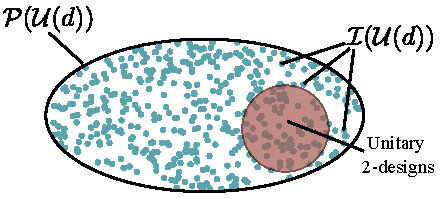
\includegraphics[width=0.9\linewidth]{figures/dense.pdf}
    \caption{\label{fig: dense}Schematic illustration of the relative positions of polynomial probability measures $\mathcal{I}(U(d))$ and unitary 2-designs within the space of probability measures $\mathcal{P}(U(d))$. The green discrete points represent elements of $\mathcal{I}(U(d))$, which are densely distributed throughout $\mathcal{P}(U(d))$, while the red region denotes the set of unitary 2-designs, concentrated in a small subset of $\mathcal{P}(U(d))$.}
\end{figure}

% Since our goal is to make a computational framework of gradient variances for general PQCs, a reasonable requirement is that the approximation of pairs of probability measures should be compatible with the variance approximation. Indeed, this can be completed via the following approximation proposition:
% \begin{proposition}
% \label{prop: approx}
% For each $R \in\mathcal{D}'( U(d))$, define the continuous test function $f_R \colon  U(d) \to \mathbb{R}$ by $f_R(U) = \langle T_R,\, g_U \rangle$,
% where
% \begin{equation}
%     g_U(V) = \operatorname{Tr}\Bigl[V\rho V^\dagger \, i\bigl[H_\ell, U^\dagger O U\bigr]\Bigr]
% \end{equation}
% and $T_R$ is the probability distribution on $ U(d)$ associated with the right unitary $U_R$. The bilinear map
% \begin{equation}
%     \operatorname{Var} \colon \mathcal{D}'( U(d)) \times \mathcal{D}'( U(d)) \longrightarrow \mathbb{R}, \quad (L,R) \longmapsto L(f_R)
% \end{equation}
% is continuous with respect to the product weak$^*$-topology. This establishes that any PQC can be approximated by a pair of polynomial probability measures with arbitrary precision~\cite{NoteDist1}.
% \end{proposition}
% By Proposition \ref{prop: approx}, the approximation of pairs of probability distributions is compatible with the variance approximation. Combining the embedding given in Eq.~\eqref{eq:embedding}, compatibility can also be applied to the set of probability measures. Since $\mathcal{I}( U(d))$ is dense in $\mathcal{P}( U(d))$, any pair of probability measures can be approximated by a pair of polynomial probability measures with a bounded deviation in gradient variance.

% We next introduce two global phase factors $e^{i\alpha}$ and $e^{i\beta}$, where $\alpha$ and $\beta$ are independent and uniformly distributed on $[0, 2\pi)$, and we define $U'_L := e^{i\alpha} U_L$ and $U'_R := e^{i\beta} U_R$, respectively. It leads to the conclusion that the corresponding probability measures $\mu_L$ and $\mu_R$ become invariant under the scalar action of the unit circle $\mathbb{S}^1$. Moreover, the variance is unchanged under the transformation, i.e. ${\rm Var}_{\theta}^{(\mu_L',\mu_R')}[\partial_\ell C] = {\rm Var}_{\theta}^{(\mu_L, \mu_R)}[\partial_\ell C]$, since the partial derivative $\partial_\ell C = i\operatorname{Tr}[U_R\rho U_R^\dagger [H_\ell, U_L^\dagger O U_L]]$ is invariant under transformations $U_R\rightarrow e^{i\alpha} U_R$ and $U_L\rightarrow e^{i\beta}U_L$. Therefore, we can make the PQC $\mathbb{S}^1$-invariant by introducing global factors without affecting the variance of the gradient at any parameter. This technique is beneficial to restrict the domain of analysis further.

% Let $\mathcal{P}( U(d))^{\mathbb{S}^1}$ denote the set of all $\mathbb{S}^1$-invariant probability measures on $ U(d)$, and $\mathcal{I}_B( U(d))$ the subset of $\mathcal{I}( U(d))$ consisting of balanced polynomial probability measures. Then the following proposition holds: 
% \begin{proposition}
%     Any complex-valued polynomial on $ U(d)$ that is invariant under the $\mathbb{S}^1$-action must be a balanced polynomial. Formally, 
%     \begin{equation}
%         \mathcal{I}( U(d))^{\mathbb{S}^1} = \mathcal{I}_B( U(d)).
%         \label{eq:inv}
%     \end{equation}
%     As a corollary, $\mathcal{I}_B( U(d))$ is dense in $\mathcal{P}( U(d)))^{\mathbb{S}^1}$.
%     \label{prop: inv}
% \end{proposition}
% Proposition~\ref{prop: inv} shows that any PQC considered above can be transformed into an $\mathbb{S}^1$-invariant form without altering its gradient variance and circuit structure. Consequently, the analysis of trainability reduces to computing the variance with respect to the associated balanced polynomial measure pair $(\mu_L, \mu_R)$\cite{NoteDist2}. 

% -----------------------------------------------------------------------------------------------
%Polynomial measures provide a computable framework for evaluating gradient variances, and we analyze their computability as follows. A polynomial $f$ on $ U(d)$ is called balanced if every monomial of $f$ belongs to the space ${\rm Hom} ( U(d), t, t)$ for some $t\in\mathbb{Z}_+$. In our proposed framework, only the balanced components of the measure contribute to the final variance. Balanced polynomials can be expanded as linear combinations of zonal polynomials $Z_{\boldsymbol\lambda}(U)$, labeled by indices ${\boldsymbol\lambda} = ({\boldsymbol\lambda}_1, {\boldsymbol\lambda}_2, \ldots,{\boldsymbol\lambda}_d)$ satisfying ${\boldsymbol\lambda}_i \in \mathbb{Z}$ and ${\boldsymbol\lambda}_1 \geq {\boldsymbol\lambda}_2 \geq \cdots \geq {\boldsymbol\lambda}_d$. Consequently, by expanding $\mathrm{d}\mu_R / \mathrm{d}\mu_H$, the variance can be decomposed into a sum of several computable components according to Eq.~\eqref{eq:var2}. Notably, when expanding the gradient variance via zonal polynomials, the orthogonality properties of zonal polynomials restrict the contributing terms to those with indices lying in the set $S = \{{\boldsymbol\lambda}: |{\boldsymbol\lambda}| = 0, |{\boldsymbol\lambda}_+| \leq 2\}$, where $|{\boldsymbol\lambda}_+|$ denotes the sum of positive entries of ${\boldsymbol\lambda}$. There are $|S| = 6$ such types of zonal polynomials, whose explicit forms are detailed in \cite{roy2009unitary}.

In the polynomial measure $\mathrm{d}\mu_R / \mathrm{d}\mu_H$, only a portion of its components contribute to the gradient variance. Every monomial in these components on $\mathcal{U}(d)$ belongs to the space $\operatorname{Hom}(\mathcal{U}(d), t, t)$ for some $t \in \mathbb{Z}_+$, and we refer to them as balanced components. Balanced components can be expanded as linear combinations of zonal polynomials $Z_{\boldsymbol\lambda}(U)$, labeled by indices ${\boldsymbol\lambda} = ({\lambda}_1, {\lambda}_2, \ldots, {\lambda}_d)$ satisfying ${\lambda}_i \in \mathbb{Z}$ and ${\lambda}_1 \geq {\lambda}_2 \geq \cdots \geq {\lambda}_d$. When the balanced components in the measure are expanded via zonal polynomials, the total gradient variance is consequently decomposed into a sum of several components. Notably, the orthogonality properties of zonal polynomials restrict the contributing terms to those with indices lying in the set $S = \{{\boldsymbol\lambda}: |{\boldsymbol\lambda}| = 0, |{\boldsymbol\lambda}_+| \leq 2\}$, where $|{\boldsymbol\lambda}_+|$ denotes the sum of the positive entries of ${\boldsymbol\lambda}$.There are $|S| = 6$ such types of zonal polynomials, whose explicit forms are detailed in \cite{roy2009unitary}.

If we further assume that each parameter satisfies $\theta_i\sim \mathrm{Uniform}[0, 2\pi)$, then the polynomial measures to approximate each component of PQC (including single rotation gates and fixed entangling gates) can be exactly obtained by the following theorem:
% \begin{theorem}
%     Let $R = \exp(iP\theta)$ be a rotation gate, where $P=\otimes_{i=1}^n\sigma_i$ is a Pauli word and $\theta\sim \mathrm{Uniform}[0, 2\pi)$. The distribution of $R$ admits an approximation by a sequence of polynomials $\{f_P^m\}_{m=1}^\infty$, where 
%     \begin{equation}
%         f_P(V) = |\operatorname{Tr}[V]|^2 + |\operatorname{Tr}[PV]|^2.
%     \end{equation}
    
%     For a fixed entangling gate $W_\ell$, its distribution is given by Dirac delta distribution
%     \begin{equation}
%         \delta_{W_\ell}(V) = \left\{\begin{aligned}
%             1,\quad &W_\ell = V\\
%             0,\quad &{\rm otherwise}
%         \end{aligned}\right. .
%     \end{equation}
%     \label{thm:comp}
% \end{theorem}
\begin{theorem}
    Let $R = \exp(iP\theta)$ be a rotation gate, where $P=\otimes_{i=1}^n\sigma_i$ is a Pauli word and $\theta\sim \mathrm{Uniform}[0, 2\pi)$. The distribution of $R$ admits an approximation by the following partial sums 
    \begin{equation}
        p_N = \frac{1}{2\pi}\int_0^{2\pi}\dif\theta\sum_{|{\boldsymbol\lambda}|\leq N}Z_{{\boldsymbol\lambda}, e^{iP\theta}},\quad N\in \mathbb{Z}_+.
    \end{equation}
    Furthermore, at the level of computing gradient variance, the distribution of $R$ is equivalent to
    \begin{equation}
        \begin{aligned}
           p_{2,b} &= 1 + \frac{1}{2}(Z_{(1,0,\cdots,0,-1),I} + Z_{(1,0,\cdots,0,-1),P})
            + \frac{1}{4}\\
            &\sum_{|{\boldsymbol\lambda}| = 0,\ |{\boldsymbol\lambda}_+| = 2}(Z_{{\boldsymbol\lambda},I} + Z_{{\boldsymbol\lambda},P} + Z_{{\boldsymbol\lambda},\frac{(I+iP)}{\sqrt{2}}} + Z_{{\boldsymbol\lambda},\frac{(I-iP)}{\sqrt{2}}}).
        \end{aligned}
    \end{equation}
    For a fixed entangling gate $W_\ell$, its distribution is given by the Dirac delta distribution concentrated at $W_\ell$.
    % \begin{equation}
    %     \delta_{W_\ell}(V) = \left\{\begin{aligned}
    %         \infty,\quad &W_\ell = V\\
    %         0,\quad &{\rm otherwise}
    %     \end{aligned}\right. .
    % \end{equation}
    \label{thm:comp}
\end{theorem}
The probability measure of the whole circuit is just the convolution of the probability measures of each component in order. Thus, we can summarize the following corollary:
% \begin{corollary}
%     Given an arbitrary PQC of the form $U(\theta) = \prod_{j=1}^L \exp(iP_j\theta_j)W_j$, this circuit can be approximated by a sequence of polynomial measures $\{\nu_m\}_{m=1}^\infty$ with derivative 
%     \begin{equation}
%         \frac{\dif\nu_m}{\dif\mu_H} = f_{P_1}^m * \delta_{W_1} * \cdots *f_{P_L}^m * \delta_{W_L}.
%     \end{equation}
%     \label{cor:approx_prac}
% \end{corollary}
\begin{corollary}
Let $U(\boldsymbol\theta) = \prod_{j=1}^L\exp(iP_j\theta_j)W_j$, where $P_j$ are Pauli words and $U\sim {\rm Uniform}[0,2\pi)$ independently. Then, the gradient variance induced by the circuit $U$ coincides with that of the polynomial $f$ defined below.
\begin{equation}
    \begin{aligned}
      f = 1 + &\frac{1}{2^{L}}\sum_{i_1,\ldots,i_L=1}^{2} Z_{(1,0,\ldots,0,-1),\,\prod_{s=1}^{L} P_s^{i_s}W_s}+\\
       &\frac{1}{4^{L}}\sum_{|{\boldsymbol\lambda}|=0,\ |{\boldsymbol\lambda}_+|=2}\sum_{i_1,\ldots,i_L=1}^{4}Z_{{\boldsymbol\lambda},\,\prod_{s=1}^{L} P_s^{i_s}W_s}.
    \end{aligned}
\end{equation}
Here, for a Pauli word $P$, we write $ P^1 := I, \ P^2 := P, \ P^3 := (I+iP)/\sqrt{2}, \ P^4 := (I-iP)/\sqrt{2}$.
\label{cor:approx_prac}
\end{corollary}
Corollary~\ref{cor:approx_prac} provides an explicit polynomial measure family to approximate any PQC under the hardware-efficient ansatz. Thus, the gradient variance of an arbitrary PQC can be obtained by the Weingarten calculus of polynomials with respect to the Haar measure.
For rigorous approximation statements and proofs of Theorem~\ref{thm:comp} and Corollary~\ref{cor:approx_prac}, one can refer to the Supplementary Materials Sec.~\RomanNumeralCaps{2}.

% -------------------------------------------------------------------------------------------
% If the rotation gate takes the form $\exp(iP\theta)$, where $\theta \sim \text{Uniform}[0, 2\pi)$ and $P$ is a Pauli word, we demonstrate that the measure of a single rotation gate can be approximated by a polynomial measure $\mu_m^P$, where a larger $m$ yields a more accurate approximation. The Radon-Nikodym derivative of this polynomial measure, which quantifies its deviation from the standard Haar measure, is given by
% \begin{equation}
%         \frac{\dif\mu_m^P}{\dif\mu_H}(U) = \left(|\operatorname{Tr}[U]|^2 + |\operatorname{Tr}[PU]|^2\right)^m.
% \end{equation}
% Practical parameterized quantum circuits consist of parameterized rotation gates and fixed entangling gates. By basic probability theory, the probability measure of the entire circuit is the convolution of the probability measures of each block in order. Therefore, for a given PQC $U(\theta) = \prod_{j=1}^L \exp(iP_j\theta_j) W_j$, where $W_j$ are entangling gates, the circuit can also be approximated by a polynomial measure $\nu_m$, with Radon-Nikodym derivative
% \begin{equation}
%         \frac{\dif\nu_m}{\dif\mu_H} = \frac{\dif\mu_m^{P_1}}{\dif\mu_H} * \delta_{W_1} * \cdots *\frac{\dif\mu_m^{P_L}}{\dif\mu_H} * \delta_{W_L}.
% \end{equation}
% where $\delta_{W_k}$ is a delta function that $\delta_{W_k}(U) = 0$ when $U \neq W_k$ and $\delta_{W_k}(U) = 1$ when $U= W_k$. For rigorous proofs of the approximation of a single gate and the whole circuit, one can refer to the Supplementary Materials Sec.~\RomanNumeralCaps{2}.
In the remaining content, we will delve deeper into the analysis of variance on the balanced polynomial measures. Since the analysis for $U_L$ and $U_R$ is analogous, without loss of generality, we focus on the right part $U_R$ in the discussion\cite{NoteDist3}. 

%\emph{Level classification of variances.}---Universal approximation of arbitrary PQCs by polynomial measures is enough to provide a computational framework for gradient variances, as gradient variances on polynomial measures can be carried out by the Weingarten calculus\cite{collins2003moments,collins2006integration}. When integrating polynomials with respect to the Haar measure, only the balanced components contribute, which allows us to restrict our analysis to balanced polynomial measures. Moreover, the derivatives of these measures admit a further decomposition in terms of zonal polynomials, leading to an exponential-level classification. We begin by reviewing the fundamental properties of zonal polynomials. 

%Any irreducible representation of the unitary group $ U(d)$ can be labeled by a non-increasing integer sequence ${\boldsymbol\lambda}:=({\boldsymbol\lambda}_1,{\boldsymbol\lambda}_2, \cdots,{\boldsymbol\lambda}_d)$ of length $d$, where ${\boldsymbol\lambda}_i\in\mathbb{Z}$ and ${\boldsymbol\lambda}_1\geq{\boldsymbol\lambda}_2\geq\cdots\geq {\boldsymbol\lambda}_d$ \cite{bump2004lie}. For each irreducible representation ${\boldsymbol\lambda}$, one can define a family of polynomials $\{Z_{{\boldsymbol\lambda}, V}: V\in U(d)\}$, known as zonal polynomials~\cite{james1961zonal,james1964distributions,constantine1963some}, which form a basis for the vector space of the balanced polynomials on $ U(d)$.  A key property of zonal polynomials is their orthogonality across distinct indices~\cite{roy2009unitary}, i.e., $\left<Z_{{\boldsymbol\lambda}, V_1}, Z_{{\boldsymbol\lambda}', V_2}\right> = \delta_{{\boldsymbol\lambda},{\boldsymbol\lambda}'}\left<Z_{{\boldsymbol\lambda}, V_1}, Z_{{\boldsymbol\lambda}, V_2}\right>$, where $\left<\cdot,\cdot\right>$ is the Hilbert-Schmidt inner product. It is known that every element in ${\rm Hom}( U(d), t, t)$ can be expressed as a linear combination of zonal polynomials in $\{Z_{{\boldsymbol\lambda}, U}: U\in U(d), |{\boldsymbol\lambda}| =0, |{\boldsymbol\lambda}_+| \leq t\}$, where ${\boldsymbol\lambda}_+$ denotes the sum of positive entries of ${\boldsymbol\lambda}$ and $|{\boldsymbol\lambda}|$ denotes the sum of all entries of ${\boldsymbol\lambda}$. Formally, any balanced polynomial of degree $t$ admits the expansion
% \begin{equation}
%     p = \sum_{|{\boldsymbol\lambda}| = 0,|{\boldsymbol\lambda}_+|\leq t}\sum_{V_{\boldsymbol\lambda}}a_{{\boldsymbol\lambda},V_{\boldsymbol\lambda}} Z_{{\boldsymbol\lambda}, V_{\boldsymbol\lambda}},
% \end{equation}
% where $a_{{\boldsymbol\lambda}, V_{\boldsymbol\lambda}}\in \mathbb{R}$ is the coefficient of each zonal polynomial $Z_{{\boldsymbol\lambda},V_{\boldsymbol\lambda}}$. By the orthogonality, it suffices to restrict attention to those zonal polynomials with indices in $S_{\leq 2}:=\{{\boldsymbol\lambda}: |{\boldsymbol\lambda}| = 0, |{\boldsymbol\lambda}_{+} |\leq 2\}$, when considering the variance problem. There are $|S_{\leq 2}| = 6$ such types of zonal polynomials, whose explicit forms are detailed in \cite{roy2009unitary}.

% We decompose the right derivative $g:= \dif\mu_R/\dif\mu_H$ as $\sum_i g_i$, where $g_i$ denotes the projection of $g$ onto the subspace $\bigoplus_{|{\boldsymbol\lambda}|=0, |{\boldsymbol\lambda}_+|=i} V_{\boldsymbol\lambda}$. The $i$-th-order variance is defined as
% \begin{equation}
%     \begin{aligned}
%         {\rm Var}^{(\mu_L,\mu_R)}_i&(\rho,O) :=\\
%         &\int\dif\mu_L(U_L)\dif\mu_H(U) g_i(U) \operatorname{Tr}[U\rho U^\dagger X_L]^2.
%     \end{aligned}
% \end{equation}
% As discussed above, it is clear that the total variance
% \begin{equation}
%     {\rm Var}^{(\mu_L,\mu_R)}_\theta(\rho,O) = \sum_{i=0}^2{\rm Var}^{(\mu_L,\mu_R)}_i(\rho, O).
% \end{equation}
% As an application of classical unitary design theory, it is known that ${\rm Var}^{(\mu_L,\mu_R)}_0(\rho, O)\leq C_0(\rho, O)d^{-2}$ for some constant $C_0(\rho, O) > 0$. In the following theorem, we will quantify the first- and second-order variances:


\emph{Level classification of variances.}--- The above analysis shows that an arbitrary PQC can be approximated by polynomial probability measures. The balanced component of such measures, which governs the gradient variance, admits a decomposition in terms of zonal polynomials~\cite{james1961zonal,james1964distributions,constantine1963some}. Consequently, the total variance can be expressed as the sum of three contributions:
\begin{equation}
    \operatorname{Var}^{(\mu_L, \mu_R)}(\rho, O) = \sum_{i=0}^2 \operatorname{Var}_i^{(\mu_L, \mu_R)}(\rho, O).
    \label{eq:var_decomp}
\end{equation}
%Based on this expansion, we decompose $g := \mathrm{d}\mu_R / \mathrm{d}\mu_H$ as $g = \sum_i g_i$, where $g_i$ denotes the projection of $g$ onto the subspace $\bigoplus_{|{\boldsymbol\lambda}|=0, |{\boldsymbol\lambda}_+|=i} V_{\boldsymbol\lambda}$, where $|{\boldsymbol\lambda}| = \sum_i {\boldsymbol\lambda}_i$, $|{\boldsymbol\lambda}_+|$ denotes the sum of positive entries of ${\boldsymbol\lambda}$ and $V_{\boldsymbol\lambda}$ is the irreducible subspace indexed by ${\boldsymbol\lambda}$. The $i$-th order variance can thus be expressed as
% \begin{equation}
%     \begin{aligned}
%         {\rm Var}^{(\mu_L,\mu_R)}_i&(\rho,O) :=\\
%         &\int\dif\mu_L(U_L)\dif\mu_H(U) g_i(U) \operatorname{Tr}[U\rho U^\dagger X_L]^2.
%     \end{aligned}
% \end{equation}
Through the zonal polynomial decomposition, we have projected the variance onto several subspaces that admit explicit computation successfully. Among these, the bound $\operatorname{Var}_0 \leq C_0(\rho,O) d^{-2}, C_0(\rho,O)>0$ for the zeroth-order variance is a well-established result. For the first- and second-order variances, we provide the following theoretical upper bounds.


\begin{theorem}
    Given a balanced probability polynomial measure $\mu_R$, the $\alpha$-th-order variance admits the following asymptotic bounds:
    \begin{equation}
        {\rm Var}^{(\mu_L,\mu_R)}_\alpha(\rho, O) \leq C_\alpha(\rho, O)d^{\alpha-2}\quad {\rm for}\ \alpha=0,1,2,
    \end{equation}
    where $C_\alpha(\rho, O)$ is a constant independent on $d$.
    \label{thm:1}
\end{theorem}
Building on the uniform approximation by polynomial measures, Theorem~\ref{thm:1} characterizes the variance contributions from each orthogonal subspace for general PQCs, which provides a level classification of total variances based on structural properties of measures. It demonstrates that the second-order variance determines whether there exists a barren plateau at the given parameter. Moreover, for a pure state $\rho$, there is a further restriction that
    \begin{equation}
        {\rm Var}^{(\mu_L,\mu_R)}(\rho, O) \leq \frac{d}{2}{\rm Var}^{(\mu_L,\mu_R)}_1(\rho, O) + \mathcal{O}(d^{-1}),
        \label{eq:upper_bound}
    \end{equation}
   indicating that a large first-order variance is necessary to avoid degraded trainability.

From Eq.~\eqref{eq:upper_bound}, we can derive that when at least one of $\mu_L$ or $\mu_R$ forms a unitary 1-design, the total variance is upper-bounded by $d^{-1}$ up to a constant. The following proposition shows the attainability of this bound.
\begin{proposition}
   Let $\nu_m$ be a probability measure on the unitary group $ U(d)$ whose derivative satisfies
\begin{equation}
    \frac{\dif\nu_m}{\dif\mu_H}(U) = c_m\operatorname{Tr}[U\rho U^\dagger P]^{2m},
    \label{eq:1-design}
\end{equation}
where $\rho$ is a pure state, $P$ is an idempotent matrix, and $c_m$ is the normalization constant. Then $\nu_m$ defines a unitary 1-design. Moreover, for sufficiently large $m$, there exists a measure $\mu_L$ and an observable $O$ such that 
\begin{equation}
    {\rm Var}^{(\mu_L,\nu_m)}(\rho, O)\geq \gamma d^{-1}
\end{equation}
for some constant $\gamma>0$.
\label{prop:1-design}
\end{proposition}
This result indicates that when the PQC forms a unitary 1-design, its total gradient variance can be at most on the order of \(d^{-1}\), thereby exhibiting superior trainability compared to unitary 2-designs, which are bounded by the $d^{-2}$ scaling. The proofs of Theorem~\ref{thm:1} and Proposition~\ref{prop:1-design} are provided in Supplementary Material, Sec.~\RomanNumeralCaps{3}.


\begin{figure}[htbp]
\centering
    \centering
    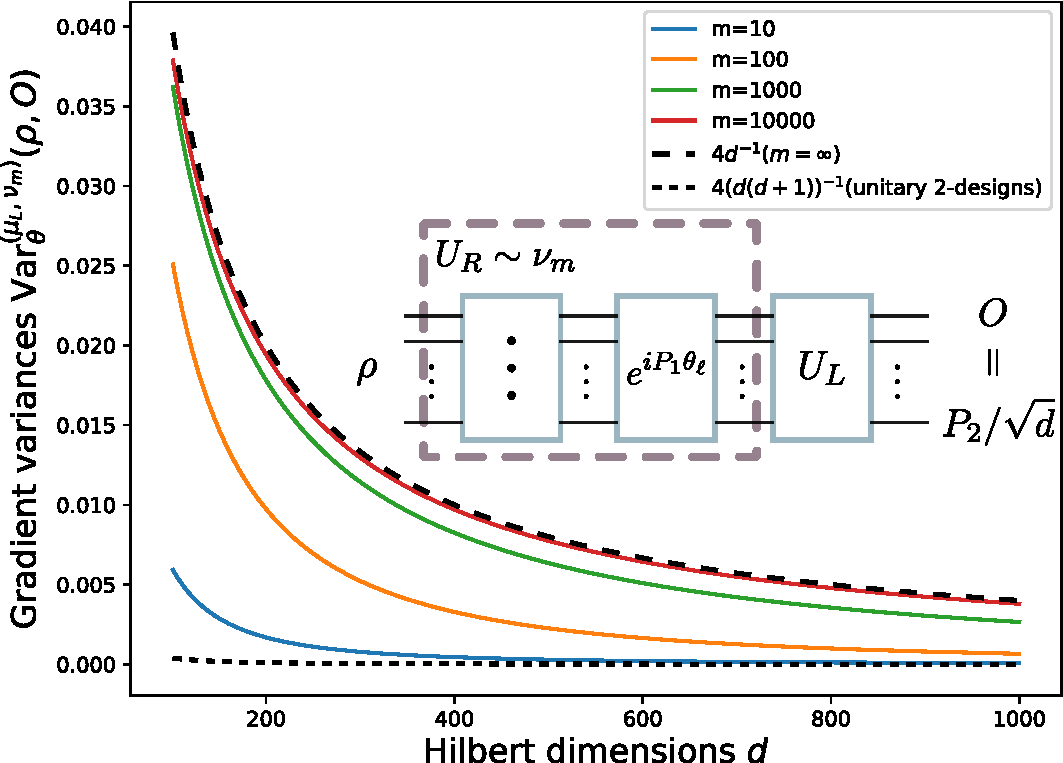
\includegraphics[width=0.96\linewidth]{figures/bound.pdf}
    \caption{The gradient variances of the circuit when adopting unitary 1-designs and unitary 2-designs as functions of the system size $d$. The inset shows the circuit structure used in this example. The long-dashed line represents the upper bound $4d^{-1}$ for unitary 1-designs in this circuit and the colored solid lines correspond to unitary 1-designs with $\mu_R$ taking different $\nu_m$. The gradient variance gradually approaches the upper bound as $m$ increases. In contrast, when the circuit adopts a unitary 2-design, the gradient variance is fixed at $4(d(d+1))^{-1}$ (short-dashed line).}
\label{fig:main1}
\end{figure}
% Furthermore, we demonstrate the attainability of the $d^{-1}$ scaling of gradient variances under the specific unitary 1-design setting. We take $O=P_1/\sqrt{d}$ and $H_\ell=P_2$, where $P_1$ and $P_2$ are two noncommuting Pauli words. For the circuit configuration, let $U_R$ be a unitary 1-design whose derivative takes the form $c_m\operatorname{Tr}[U\rho U^\dagger P]^{2m}$, where $P$ satisfies $[P_1,P_2]=2iP$, while $U_L$ commutes with $O$. Under these conditions, our theoretical result shows that gradient variances scale as $d^{-1}$ when $m$ is sufficiently large, significantly outperforming the $d^{-2}$ scaling of unitary 2-designs, as illustrated in Figure~\ref{fig:main1}.
Furthermore, we demonstrate the attainability of the $d^{-1}$ scaling of the gradient variance at a given parameter $\theta_\ell$ under a specific unitary 1-design setting. Consider the rotation gate at position $\theta_\ell$ to be $\exp(iP_1\theta_\ell)$ and the observable $O = P_2/\sqrt{d}$, where $P_1$ and $P_2$ are two noncommuting Pauli words and $U_L$ is an operator commuting with $P_2$. When $U_R$ forms a unitary 2-design, the variance ${\rm Var}^{(\mu_L, \mu_R)}(\rho, O)$ can be computed as $4(d(d+1))^{-1}$, as indicated by the short-dashed line in Figure ~\ref{fig:main1}. When $U_R$ is taken as the unitary 1-design satisfying Eq.~(9) with $[P_1, P_2] = 2iP$, the variance ${\rm Var}^{(\mu_L, \mu_R)}(\rho, O)$ is bounded by the $d^{-1}$ scaling and, as $m$ increases (colored solid lines in Figure 2), approaches the upper bound $4d^{-1}$, marked by the long-dashed line.
%Since unitary 1-designs exhibit weaker randomness, they provide a more suitable assumption for modeling trainable PQCs than unitary 2-designs. In Proposition~\ref{prop:1-design}, we construct an explicit family of probability measures that form unitary 1-designs and attain the upper bound on the total variance. This result demonstrates that unitary 1-designs can achieve superior trainability compared to unitary 2-designs. The proofs of Theorem~\ref{thm:1} and Proposition~\ref{prop:1-design} are provided in Supplementary Material, Sec.~\RomanNumeralCaps{3}.

\emph{The Improvement Potential.}--- So far, several methods have been developed to enhance trainability, such as the substitution by shallow circuits, tailored problem-specific ansatz, and optimized initialization strategies~\cite{zhang2024absence,cerezo2021cost, liu2024mitigating, grant2019initialization}. However, these approaches typically rely on global or heuristic modifications and provide limited quantitative guidance within a fixed circuit structure. Here, we propose a formula to characterize the maximal improvement of trainability through inserting oracles adjacent to a given position. Specifically, we insert a parametric oracle $S_p$ associated with the probability measure $\mu$ on the left side of $U_R$. The probability measure for the combination of $U_R$ and $S_p$ is the convolution $\mu * \mu_R$. The schematic diagram of the process is shown in Figure~\ref{fig: circuit}.

\begin{figure}[htbp]
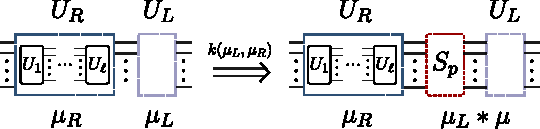
\includegraphics[width=0.9\linewidth]{figures/circuit.pdf}
\caption{\label{fig: circuit} The process of inserting oracles adjacent to the given position to potentially enhance trainability. Here, $S_p$ denotes an arbitrary unitary oracle associated with probability measure $\mu$ and the improvement potential $k_{\mu_R}$ represents the maximal improvement of the total variance during the process.}
\label{fig:insert}
\end{figure}
Formally, we consider the following quantity
\begin{equation}
    k_{\mu_R} : = \sup_{\mu\in\mathcal{P}( U(d))}\frac{{\rm Var}^{(\mu_L, \mu*\mu_R)}(\rho, O)}{{\rm Var}^{(\mu_L,\mu_R)}(\rho, O)},
\end{equation}
which characterizes the maximal relative enhancement of variance at the parameter $\theta_\ell$ by inserting an oracle. If $k_{\mu_R}=1$, the PQC exhibits no improvement potential at $\theta_\ell$; whereas $k_{\mu_R}>1$ indicates the existence of improvement potential at that parameter. We provide the following criterion to determine whether $k_{\mu_R}>1$ or not:
\begin{theorem}
For a PQC at $\theta_\ell$ with the probability measure pair $(\mu_L, \mu_R)$, the improvement potential obtained by inserting an oracle is
\begin{equation}
    k_{\mu_R}  = \frac{\|g*h\|_\infty}{\|gh\|_1}.
\end{equation}
Here $g$ and $h$ are functions on $U(d)$ defined by
\begin{equation}
    g(V) = \frac{\dif \mu_R}{\dif \mu_H}(V), h(V) = \int \dif \mu_L(U_L)\,
    \operatorname{Tr}\!\left[V^\dagger \rho V X_L\right]^2 .
\end{equation}
The function $g$ denotes the derivative of $\mu_R$ with respect to $\mu_H$, while $h$ represents the variance obtained after integrating over the left unitary. Both functions can be decided by the pair $(\mu_L,\mu_R)$.
\label{thm:potential}
\end{theorem}
Moreover, we find that the quantity ${\rm Var}^{(\mu_L, \mu_H)}(\rho, O)$ can serve as a reference threshold for determining whether improvement potential exists at a given parameter, where this value corresponds to the unitary 2-design case. For a pair of probability measures $(\mu_L, \mu_R)$, if ${\rm Var}^{(\mu_L, \mu_R)}(\rho, O) < {\rm Var}^{(\mu_L, \mu_H)}(\rho, O)$, then the pair possesses improvement potential. In contrast, for circuits where $\mu_R$ satisfies the unitary 2-design property, the gradient variance satisfies ${\rm Var}^{(\mu_L, \mu_R)}(\rho, O) = {\rm Var}^{(\mu_L, \mu_H)}(\rho, O)$. However, such circuits exhibit no training potential, i.e., $k_{\mu_R} = 1$. Therefore, all parameterized quantum circuits, after being optimized through the process illustrated in Figure~\ref{fig:insert}, can achieve performance at a given parameter position that is no worse than that of unitary 2-design circuits. When $\operatorname{Var}^{(\mu_L, \mu_R)}(\rho, O) \geq \operatorname{Var}^{(\mu_L, \mu_H)}(\rho, O)$, no definitive conclusion can be drawn from this comparison alone. In this regime, the presence or absence of improvement potential must be determined using the criterion established in Theorem~\ref{thm:potential}.More detailed discussions and constructive examples are provided in the Supplementary Material Sec.~\RomanNumeralCaps{4}.

%If we define the potential training ability of a parameterized quantum circuit as the optimal training performance achievable through the process illustrated in Figure~\ref{fig: circuit}, then circuits with a unitary 2-design property exhibit the lowest potential training ability among all parameterized quantum circuits. When ${\rm Var}^{(\mu_L, \mu_R)}_\theta(\rho, O) \geq {\rm Var}^{(\mu_L, \mu_H)}_\theta(\rho, O)$, no definitive conclusion can be drawn from this comparison alone. In this regime, the presence or absence of improvement potential must be determined using the criterion established in Theorem~\ref{thm:potential}.

% As an explanation, we construct two specific classes of probability measure pairs that make this situation clearer. First, we construct a family of pairs $(\mu_L, \mu_R)$ that simultaneously exhibit poor trainability at the given parameter and no improvement potential, demonstrating that certain poorly trainable networks also lack improvement potential. Second, we demonstrate that there also exists a poorly trainable $(\mu_L, \mu_R)$ with a maximal achievable improvement potential up to $d$-scaling.
% \begin{proposition}
% For a PQC generated by a pairwise non-commuting set $\{H_i\}_{i=0}^L$, there exists a pure state $\rho = \left|\phi\right>\left<\phi\right|$ and a normalized state $\left|\psi\right>$ such that, if the measure $\mu_R$ is defined by
%     \begin{equation}
%         \frac{\dif\mu_R}{\dif\mu_H}(U) = \begin{pmatrix} m+d-1\\ d-1
%     \end{pmatrix}\operatorname{Tr}[U\rho U^\dagger\left|\psi\right>\left<\psi\right|]^{2m},
%     \end{equation}
% the improvement potential of $(\mu_L,\mu_R)$ can attain order $d^2$ for all $m\in \Omega(d)$.
% \end{proposition}
% It characterizes the maximal achievable improvement potential under this framework.
% For details of the above statements, we refer readers to the Supplementary Material Sec.~\RomanNumeralCaps{4}.

\emph{\label{sec:5} Numerical Simulation.}---To validate our theory, we perform numerical simulations using Monte Carlo methods for circuits satisfying the unitary 1-design condition, computing the total gradient variance at the parameter $\theta_\ell$, and compare the results with the theoretical predictions given by our polynomial method. The simulated circuit structure is illustrated in Figure~\ref{fig:num}a, where $U_R$ is a universal block constructed following the approach in \cite{tilma2002parametrization, tilma2002generalized}, with its measure derivative satisfying Eq.~\eqref{eq:1-design}. The left unitary $U_L = \exp(iP'\beta)$ is an arbitrary rotation gate, where $P'$ denotes a Pauli word. 

% \begin{figure}[htbp]
%     \begin{subfigure}[b]{\linewidth}
%         \caption{\label{fig:sub1}}
%         
\includegraphics[width=0.96\linewidth]{cir_str_c.pdf}
%     \end{subfigure}
%     \begin{subfigure}{0.48\linewidth}
%     \caption{\label{fig:sub2}}
%     \centering
%     \includegraphics[width=\linewidth]{unitary_1_design_example_3bits_1.pdf}
% \end{subfigure}
% \hfill
% \begin{subfigure}{0.48\linewidth}
%     \caption{}
%     \centering
%     \includegraphics[width=\linewidth]{unitary_1_design_example_3bits_3.pdf}
%     \label{fig:sub3}
% \end{subfigure}
%     \caption{\label{fig:cir} Simulation setup and validation results. (a) The quantum circuit used in simulations. Here, $G_k$ and $D_k$ represent rotation gates of different structures and the gradient variance is evaluated at $D_{d-1}$. See Supplemental Material Sec.~\RomanNumeralCaps{5} for detailed parameter configurations. (b), (c) The correlation of theoretical predictions of gradient variance obtained from our method and Monte Carlo estimates on a three-qubit system with the observable $O = Z\otimes I\otimes Z$ and the initial pure state $\rho = \left|0\right>\left<0\right|$. Each point corresponds to a different value of the polynomial degree $2m$ and the dashed line is $y=x$, which indicates perfect agreement. In (b), $P = X\otimes Z\otimes Z$. In (c), $P = Z\otimes Z\otimes Z$.}
% \end{figure}
\begin{figure}[htbp]
    \centering
    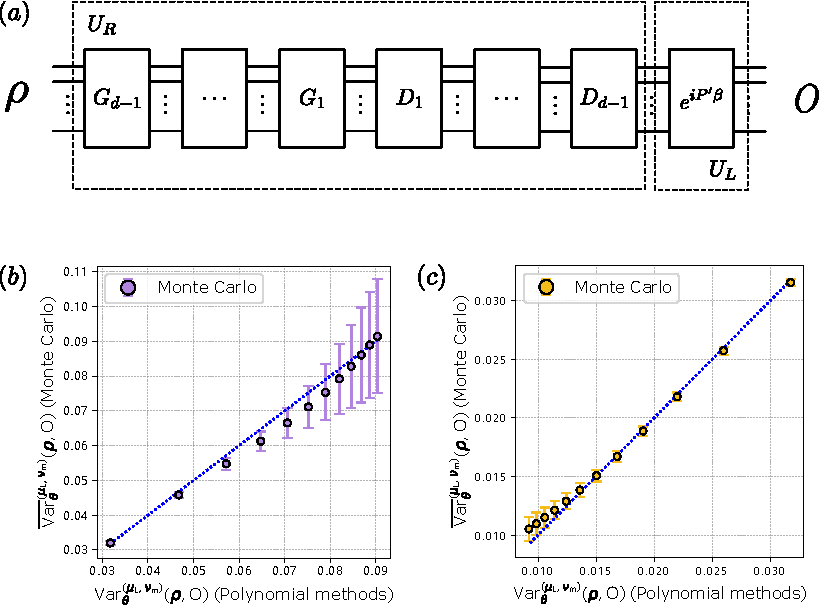
\includegraphics[width=0.96\linewidth]{figures/cir&num.pdf}
    \caption{\label{fig:num} Simulation setup and validation results. (a) The quantum circuit used in simulations. Here, $G_k$ and $D_k$ represent rotation gates of different structures and the gradient variance is evaluated at $D_{d-1}$. See Supplemental Material Sec.~\RomanNumeralCaps{5} for detailed parameter configurations. (b), (c) The correlation of theoretical predictions of gradient variance obtained from our method and Monte Carlo estimates on a three-qubit system with the observable $O = Z\otimes I\otimes Z$ and the initial pure state $\rho = \left|0\right>\left<0\right|$. Each point corresponds to a different value of the polynomial degree $2m$ and the dashed line is $y=x$, which indicates perfect agreement. In (b), $P = X\otimes Z\otimes Z$. In (c), $P = Z\otimes Z\otimes Z$.}
\end{figure}

% \begin{figure*}[htbp]
%     \begin{subfigure}[htbp]{0.48\textwidth}
%         \caption{\label{fig:main_3bits}}
%         \includegraphics[width=0.8\linewidth]{unitary_1_design_example_3bits.pdf}
%     \end{subfigure}
%     \begin{subfigure}[htbp]{0.48\textwidth}
%         \caption{\label{fig:main_bound}}
%         
\includegraphics[width=0.8\linewidth]{bound.pdf}
%     \end{subfigure}
%     \caption{(a) Variances of the gradient at the fixed parameter on a three-qubit system with the observable $O = Z\otimes I\otimes Z$ and the initial pure state $\rho = \left|0\right>\left<0\right|$. Different choices of Pauli words for the left unitaries are indicated in the legend. (b)Variance of the gradient approaching the $d^{-1}$ scaling as $m$ increases; see \emph{Numerical Simulation} for details of the setting. }
% \end{figure*}
Although our theory applies to circuits of arbitrary size, numerical verification is restricted to the three-qubit case due to the computational complexity of Monte Carlo methods. 
Figures~\ref{fig:num}b and~\ref{fig:num}c show correlation plots of a series of the theoretical gradient variances $\operatorname{Var}^{(\mu_L,\nu_m)}(\rho, O)$ and the Monte Carlo estimates $\overline{\operatorname{Var}}^{(\mu_L,\nu_m)}(\rho, O)$, both obtained by varying the balanced polynomial degree $2m$ of $\nu_m$ for two different choices of $U_L$.
%Figures~\ref{fig:sub2} and~\ref{fig:sub3} show correlation plots between the theoretical gradient variances $\operatorname{Var}_\theta^{(\mu_L,\mu_R^m)}(\rho,O)$ and the Monte Carlo estimates $\overline{\operatorname{Var}}_\theta^{(\mu_L,\mu_R^m)}(\rho,O)$ for two different choices of $U_L$ ($P=XXZ$ and $P=ZZZ$), obtained by varying the balanced polynomial degree $2m$ of $\mu_R^m$. 
The theoretical values are computed using our polynomial method, while the estimates are obtained via Monte Carlo simulation. In both cases, the data points cluster tightly around the line $y=x$, and the differences between the theoretical values and the estimates are within one standard deviation, showing excellent agreement.



%However, the practical implementation of numerical simulations becomes increasingly challenging as $n$ grows, due to the exponential increase in the number of Monte Carlo samples required for convergence. For instance, $10^8$ samples were used for the two-qubit case, whereas more than $10^{12}$ samples would be required to achieve the same precision for three qubits. For larger $n$, the number of samples necessary to maintain precision becomes enormous. In contrast, our theoretical results remain valid and accurate for all values of $m$, which are currently beyond the reach of numerical simulations.

Trainability plays a central role in the optimization of PQCs, as it determines whether circuit parameters can be efficiently updated. In this Letter, we introduce a measure-theoretic framework based on balanced polynomial measures to characterize the trainability of PQCs. We show that balanced polynomial measures can approximate any PQC with arbitrary precision up to a global factor. Within this framework, we propose a level classification of trainability based on zonal polynomial decomposition. As an application, we rigorously demonstrate that unitary 1-designs can exhibit superior trainability compared to unitary 2-designs. These theoretical findings are further supported by numerical simulations. Furthermore, we introduce the concept of improvement potential and identify a reference threshold for determining whether the trainability of a circuit possesses such potential, and present illustrative examples for different scenarios. Our work reveal internal factors that govern trainability and provide guiding principles for designing more trainable PQCs. Future research may benefit from the decomposition of the space that circuits occupy using dynamic Lie algebras~\cite{diaz2023showcasing, ragone2024lie}, which could provide a more practical and structurally informed framework for achieving more precise approximations.
\bibliography{ms}% Produces the bibliography via BibTeX.
\end{document}